\documentclass[11pt,a4paper]{article}

% --- Packages ---
\usepackage[utf8]{inputenc}
\usepackage[T1]{fontenc}
\usepackage{lmodern}
\usepackage{microtype}
\usepackage[margin=1in]{geometry}
\usepackage{amsmath,amssymb}
\usepackage{booktabs}
\usepackage{tabularx}
\usepackage{float}
\usepackage{enumitem}
\usepackage{tikz}
\usetikzlibrary{shapes.geometric, arrows.meta, positioning, calc}
\usepackage[colorlinks=true, linkcolor=blue!70!black, citecolor=blue!70!black, urlcolor=blue!70!black]{hyperref}

% --- Prevent widows, orphans, and broken hyphenations ---
\widowpenalty=10000
\clubpenalty=10000
\hyphenpenalty=5000
\exhyphenpenalty=5000

% --- Custom Column Type for Tabularx ---
\newcolumntype{Y}{>{\raggedright\arraybackslash}X}

% --- Title & Author ---
\title{\textbf{Decompose, Then Decide: A Fixer-Guided Harness for Reliable Offline Code Repair with Gemma 4 E4B}}
\author{\textbf{Naman Jain}}
\date{}

\begin{document}

\maketitle

\begin{abstract}
\noindent Small open models like Gemma 4 E4B fail at repository-level repair not because they cannot write code, but because free-form agent loops overload them with simultaneous exploration, context management, and decision-making, yielding a 14.6\% resolve rate \cite{LOOP}. Two independent research threads have attacked this bottleneck in isolation. Harness decomposition structures the repair loop into explicit stages and raises that resolve rate to 45.7\% \cite{LOOP}. Fixer-Guided Localization (FGL) trains a localizer against the downstream fixer's verified-patch likelihood, letting the fixer find bugs as often as a teacher model while using 27.5\% less code \cite{FGL}. Neither has been combined. We propose a framework that unifies these insights by treating harness decomposition as a training signal: the localizer is trained inside a decomposed four-stage repair harness (localize $\rightarrow$ reproduce $\rightarrow$ patch $\rightarrow$ verify), using the frozen fixer's verified-patch likelihood as the reward. We formalize this interaction as $R = L \times S$---where localizer precision ($L$) and conditional fixer success ($S$) reinforce one another in a virtuous cycle---and distinguish synergistic amplification from a purely additive baseline. We do not claim completed experimental validation. Instead, we specify a falsifiable protocol executable on a single consumer GPU with no reinforcement learning infrastructure and no cloud APIs, and state the exact conditions under which both the effectiveness and synergy hypotheses fail.
\end{abstract}

\section{Introduction}

\subsection{Problem}
Much of today's reliable agentic code repair depends on proprietary cloud APIs and large reinforcement learning clusters, which places it out of reach for offline, consumer-hardware settings. Small open models offer an alternative, but deploying them in a free-form loop creates a context-management bottleneck: a quantized Gemma 4 E4B achieves only a 14.6\% resolve rate \cite{LOOP}. The failure is not poor code generation but poor navigation---hallucinated paths, wasted context, and loops that never reach a patch attempt.

\subsection{Gap}
Two lines of work attack this independently. Harness decomposition isolates the repair process into explicit stages and raises Gemma 4 E4B's resolve rate from 14.6\% to 45.7\% \cite{LOOP}. FGL trains the localizer against downstream fixer success rather than human relevance labels, letting the fixer find bugs as often as a teacher while using 27.5\% less code \cite{FGL}. Neither has been combined, and the separation is not incidental. Once localization and patching are distinct stages, the localizer's output is consumed by exactly one downstream component, and that component already emits a binary, machine-checkable signal---whether the patch passed its test. Structurally separating the stages therefore creates a natural opening to train the localizer on that signal rather than on human relevance labels. FGL exploits this opening inside a free-form loop; harness decomposition, meanwhile, has been used only at inference time, never as a source of training signal.

\subsection{Thesis}
We propose that the harness itself is a training signal. Training the localizer inside a decomposed repair harness, with the downstream frozen fixer's verified-patch likelihood as the reward, is expected to produce a virtuous cycle that improves localization precision and resolve rate while remaining runnable on a single consumer GPU.

\subsection{Contributions}
\begin{itemize}[leftmargin=*, nosep, topsep=4pt]
    \item \textbf{C1 (Methodological):} A unified training framework that embeds Fixer-Guided Localization inside a decomposed four-stage repair harness (localize $\rightarrow$ reproduce $\rightarrow$ patch $\rightarrow$ verify).
    \item \textbf{C2 (Empirical prediction):} The unified method will match or exceed the decomposed-harness baseline's resolve rate while using less code context than FGL trained in a free-form loop.
    \item \textbf{C3 (Practical):} A concrete, single-consumer-GPU training protocol that requires no reinforcement learning infrastructure and no cloud APIs, making reliable agentic repair accessible offline.
\end{itemize}

\section{Related Work}

Recent work addressing automated software repair emphasizes the necessity of structured agent loops to mitigate the capacity limits of smaller language models. When executing a free-form loop, smaller architectures are rapidly overwhelmed by context size and decision-making requirements. Dente et al.\ \cite{LOOP} demonstrate that a Gemma 4 E4B free-form loop resolve rate of 14.6\% improves significantly to 45.7\% when executed inside a decomposed repair harness. A similar capability gain is observed with the Gemma 4 E2B model, where performance jumps from 5.0\% to 27.4\% \cite{LOOP}. Furthermore, hybrid approaches utilizing stronger localizers or reproducers alongside small-model edits achieve resolve rates of 39.8\% and 53.7\% \cite{LOOP}. However, whether a system relies on a human-engineered pipeline or prompts a model to iteratively refine its own scaffold at inference time, purely structural approaches treat model weights as frozen rather than optimizing stage components via downstream verification signals.

Parallel to harness engineering, representation learning has improved repository navigation through Fixer-Guided Localization (FGL) \cite{FGL}. Trained on a scale of 1,629 test-verified Kimi K3 trajectories \cite{FGL}, FGL optimizes search by prioritizing files that maximize the downstream verified-patch likelihood. Evaluated under an 8-minute budget constraint \cite{FGL}, the approach allows the fixer to find the bug as often as a teacher model while using 27.5\% less code \cite{FGL}. On their development set, agents using FGL reached a patch on 53 tasks compared to 46 for a matched control, and successfully solved 8 tasks versus 6 \cite{FGL}. Moreover, FGL prevented agents from stalling; tasks stuck reading non-existent files dropped to 43 versus 54 \cite{FGL}. Consequently, FGL trained agents explore ${\sim}3\times$ more than the base model \cite{FGL}, enabling a single agent to solve up to 11 of 78 tasks \cite{FGL}.

Beyond learning-based localization, static analysis provides algorithmic context pruning for repository-scale operations. Pokhrel \cite{TOPAZ} introduces TOPAZ, evaluated against the competition public development set size of 129 tasks \cite{KAGGLE} spanning the FastAPI, Requests, Rich, and HTTPX repositories \cite{KAGGLE}. TOPAZ achieves an AST graph construction time of $< 5$ milliseconds \cite{TOPAZ} and utilizes a Personalized PageRank (PPR) restart parameter of $\alpha = 0.85$ \cite{TOPAZ} to identify relevant execution subgraphs. The resulting prompt strategy builds a focal context where focal nodes equal the full source code, while context nodes are reduced to collapsed one-line signatures \cite{TOPAZ}. While computationally efficient, such static pruning lacks the dynamic, task-specific adaptability of a learned localizer.

Despite these distinct advancements, no prior work trains a localizer inside a decomposed repair harness using the downstream fixer's verified-patch likelihood as the primary reward signal. Unifying Fixer-Guided Localization (FGL) with a decomposed framework proposes a virtuous cycle: improved localization minimizes context bloat, which directly increases the verified-patch likelihood, ultimately feeding back a cleaner training signal to the localizer.

\section{Method}

\subsection{The Decomposed Repair Harness}
To address the limitations of a free-form loop, which overloads small models with simultaneous exploration, context management, and decision-making, we utilize a decomposed repair harness \cite{LOOP}. This harness strictly isolates repository-level repair into four sequential stages: localize, reproduce, patch, and verify.

\begin{itemize}[leftmargin=*, topsep=4pt, itemsep=4pt]
    \item \textbf{Stage 1: Localize.} \emph{Input:} the user issue description and the raw repository environment. \emph{Output:} a focal context isolating the specific files, classes, and functions implicated in the bug. \emph{Failure mode:} the agent hallucinates file paths, gets stuck reading non-existent files, or retrieves an incomplete focal context, preventing downstream stages from accessing the necessary code.
    \item \textbf{Stage 2: Reproduce.} \emph{Input:} the focal context and the user issue description. \emph{Output:} an executable test script that predictably fails on the buggy codebase and is intended to pass once the bug is resolved. \emph{Failure mode:} the generated test script contains syntax errors, fails to execute due to missing environmental dependencies, or trivially passes on the broken codebase without capturing the underlying issue.
    \item \textbf{Stage 3: Patch.} \emph{Input:} the focal context, the issue description, and the failing reproduction test. \emph{Output:} a candidate code patch intended to modify the repository and resolve the user issue. \emph{Failure mode:} the model writes syntactically invalid code, modifies the wrong variables, or introduces regressions that break other components within the focal context.
    \item \textbf{Stage 4: Verify.} \emph{Input:} the candidate code patch and the reproduction test script. \emph{Output:} a binary success or failure signal based on test execution, yielding a verified patch if successful. \emph{Failure mode:} the test environment crashes, the patch times out during execution, or the patch fails the reproduction test, necessitating a rollback.
\end{itemize}

\subsection{Fixer-Guided Localization Inside the Harness}
Within this decomposed repair harness, we integrate Fixer-Guided Localization to optimize the localization stage based on downstream utility \cite{FGL}. Instead of training the localizer to mimic human relevance labels---which often include extraneous context or omit subtle algorithmic dependencies required by an AI---we train the localizer using the actual success of the patch stage.

The training objective operates sequentially: the localizer first proposes multiple candidate focal contexts for a given issue. These candidate localizations are then passed forward through the decomposed repair harness. At the patch stage---where a frozen fixer model is strictly prevented from updating its weights---the fixer attempts to generate a code patch for each proposed focal context. Finally, the verify stage executes the tests to determine if the proposed patch successfully resolves the issue.

The localizer is subsequently trained by weighting its proposed candidate localizations according to their verified-patch likelihood \cite{FGL}. Candidates that lead the frozen fixer to generate a verified patch receive high reward weights, whereas candidates that lead to patching failures---even if they visually resemble human-annotated diffs---receive low reward weights. By optimizing directly for verified-patch likelihood, the localizer learns to extract exactly the code required by the downstream fixer.

\subsection{Formalizing the Proposed Virtuous Cycle}
Because stage separation gives the localizer exactly one downstream consumer, and that consumer already emits a binary test signal, we can decompose the resolve rate into two independent factors rather than treating it as a single, opaque quantity.

We propose that embedding Fixer-Guided Localization within a decomposed repair harness instantiates a virtuous cycle. This is a proposed mechanism, not a currently demonstrated empirical result. To make it rigorously testable, we decompose the overall resolve rate ($R$) into two measurable quantities:
\begin{equation}
    R = L \times S, \quad \text{where } L = P(\text{fix site} \in \text{focal context}), \quad S = P(\text{verified patch} \mid \text{fix site} \in \text{focal context})
\end{equation}
Here, $L$ denotes \emph{localizer precision} (the fraction of proposed focal contexts that contain the true bug location), and $S$ denotes \emph{conditional fixer success} (the probability that the frozen fixer generates a test-verified patch given a valid focal context).

In a free-form loop, $S$ is depressed because the model frequently fails due to unstructured exploration errors or tool misuses before it even attempts to write a patch, producing a sparse and noisy reward signal for $L$. Executing training inside a decomposed repair harness isolates localization from patching, raising $S$ by shielding the frozen fixer from exploration burdens \cite{LOOP}. Under the virtuous-cycle hypothesis, a higher $S$ yields denser, lower-variance verified-patch likelihood weights during training, which drives a steeper improvement in $L$ than free-form FGL can achieve. In turn, cleaner focal contexts with reduced token bloat further elevate $S$ at inference time, compounding $R = L \times S$ beyond a purely additive combination.

\paragraph{Operationalizing $L$ and $S$.}
Every SWE-bench task includes a gold patch. We define the \emph{fix site} as the set of functions touched by that patch. For each task $i$, the localizer proposes $k = 4$ candidate focal contexts $\{\pi_{ij}\}_{j=1}^{k}$. We estimate localizer precision and conditional fixer success directly from these proposals:
\begin{align}
    L &= \frac{1}{Nk}\sum_{i=1}^{N}\sum_{j=1}^{k} \mathbf{1}[\text{fix site}_i \in \pi_{ij}], \\
    S &= \frac{\sum_{ij} \mathbf{1}[\text{fix site}_i \in \pi_{ij}] \cdot \mathbf{1}[\text{verified patch}_{ij}]}{\sum_{ij} \mathbf{1}[\text{fix site}_i \in \pi_{ij}]}.
\end{align}
$S$ is estimated only over proposals whose focal context contains the fix site, so the two metrics are not redundant: $L$ measures \emph{reach}; $S$ measures \emph{conversion given reach}. A localizer that returns the whole repository would achieve $L = 1$ but collapse $S$; a localizer that returns one arbitrary function maximizes neither. The identity $R = L \times S$ is therefore exact rather than approximate, and both factors are measurable from a single evaluation run.

\begin{figure}[H]
\centering
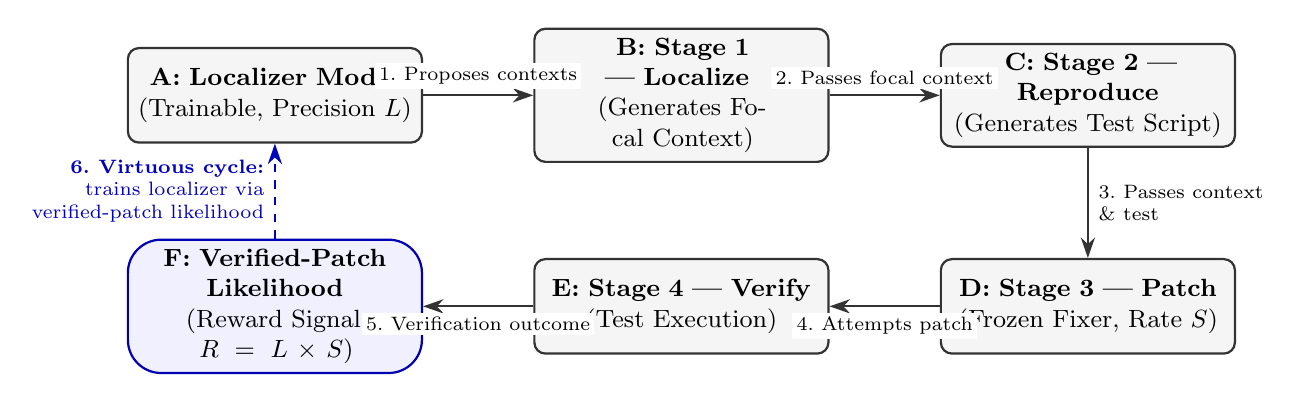
\begin{tikzpicture}[
    node distance=1.1cm and 1.4cm,
    box/.style={
        rectangle, rounded corners=4pt, draw=black!80, thick,
        fill=gray!8, text width=3.5cm, minimum height=1.2cm,
        align=center, font=\small
    },
    reward/.style={
        rectangle, rounded corners=12pt, draw=blue!70!black, thick,
        fill=blue!6, text width=3.5cm, minimum height=1.2cm,
        align=center, font=\small
    },
    arrow/.style={-{Stealth[length=2.6mm, width=1.8mm]}, thick, draw=black!80},
    dashedarrow/.style={-{Stealth[length=2.6mm, width=1.8mm]}, thick, dashed, draw=blue!75!black},
    lbl/.style={font=\scriptsize, fill=white, inner sep=1.5pt}
]

\node[box] (A) {\textbf{A: Localizer Model}\\(Trainable, Precision $L$)};
\node[box, right=of A] (B) {\textbf{B: Stage 1 --- Localize}\\(Generates Focal Context)};
\node[box, right=of B] (C) {\textbf{C: Stage 2 --- Reproduce}\\(Generates Test Script)};

\node[box, below=1.4cm of C] (D) {\textbf{D: Stage 3 --- Patch}\\(Frozen Fixer, Rate $S$)};
\node[box, left=of D] (E) {\textbf{E: Stage 4 --- Verify}\\(Test Execution)};
\node[reward, left=of E] (F) {\textbf{F: Verified-Patch Likelihood}\\(Reward Signal $R = L \times S$)};

\draw[arrow] (A) -- node[lbl, above=2pt] {1.\ Proposes contexts} (B);
\draw[arrow] (B) -- node[lbl, above=2pt] {2.\ Passes focal context} (C);
\draw[arrow] (C) -- node[lbl, right=2pt, align=left] {3.\ Passes context\\\& test} (D);
\draw[arrow] (D) -- node[lbl, below=2pt] {4.\ Attempts patch} (E);
\draw[arrow] (E) -- node[lbl, below=2pt] {5.\ Verification outcome} (F);

\draw[dashedarrow] (F) -- node[lbl, left=2pt, align=right, text=blue!75!black] {\textbf{6.\ Virtuous cycle:}\\trains localizer via\\verified-patch likelihood} (A);

\end{tikzpicture}
\caption{The proposed unified training framework embedding Fixer-Guided Localization inside a decomposed repair harness. The localizer proposes candidate contexts ($L$), which pass through reproduce and patch stages ($S$). The verification outcome establishes the verified-patch likelihood, routing back to train the localizer.}
\label{fig:framework}
\end{figure}

\section{Experimental Protocol}

\subsection{Benchmarks and Hardware}
To evaluate the proposed hypotheses, we employ two datasets. Initial validation and iterative testing are conducted on the competition public development set, consisting of 129 tasks \cite{KAGGLE}. The primary external evaluation is performed on SWE-bench Lite \cite{SWEBENCHLITE}, a widely adopted repository-level repair benchmark \cite{SWEBENCH}.

To ensure reliable agentic repair remains broadly accessible, all experiments are strictly constrained to a single consumer GPU. The base model across all configurations is a quantized \texttt{gemma-4-e4b-it}. Crucially, the training and inference pipelines require no reinforcement learning infrastructure and no external cloud APIs.

\subsection{Baselines}
We compare four empirical configurations plus an analytical additive reference (B5) to isolate whether training a localizer inside a decomposed repair harness produces synergistic interaction rather than merely additive gains:

\begin{itemize}[leftmargin=*, topsep=4pt, itemsep=3pt]
    \item \textbf{B1: Free-form loop baseline.} The base model operating in an unstructured environment. Anchors the baseline capabilities of Gemma 4 E4B, which achieves a 14.6\% resolve rate in this setting \cite{LOOP}.
    \item \textbf{B2: Decomposed repair harness baseline.} The base model operating within the sequential four-stage harness with an untrained localizer. Isolates the zero-shot architectural benefit of the decomposed repair harness, which elevates the resolve rate to 45.7\% \cite{LOOP}.
    \item \textbf{B3: FGL in a free-form loop.} A model utilizing Fixer-Guided Localization trained and evaluated entirely within a free-form loop. This acts as our control for the training signal isolated from the structured harness. B3 uses the publicly released FGL adapters.
    \item \textbf{B4: Unified method (Proposed).} An FGL model trained and evaluated inside the decomposed repair harness. B4 requires a fresh training run inside the harness and cannot be obtained by redeploying the FGL adapters used in B3.
    \item \textbf{B5: Additive reference (Analytical).} The expected resolve rate if harness decomposition and FGL combine without interaction, computed post-hoc from the observed B1, B2, and B3:
    \[
        B5 = \sigma\!\left(\operatorname{logit}(B2) + \operatorname{logit}(B3) - \operatorname{logit}(B1)\right),
    \]
    where $\sigma(x) = 1/(1+e^{-x})$ and $\operatorname{logit}(p) = \ln\!\big(p/(1-p)\big)$. B5 encodes the null hypothesis that the decomposed-harness gain and the FGL gain add on the log-odds scale with no interaction---i.e., that $S(B4) = S(B2)$ and $L(B4) = L(B3)$.
\end{itemize}

\begin{table}[H]
\centering
\caption{Baseline Configurations}
\label{tab:baselines}
\vspace{4pt}
\begin{tabularx}{\textwidth}{l l l Y}
\toprule
\textbf{Condition} & \textbf{Localizer Strategy} & \textbf{Harness Environment} & \textbf{Expected Resolve Rate} \\
\midrule
\textbf{B1} & Untrained & Free-form loop & 14.6\% \cite{LOOP} \\
\textbf{B2} & Untrained & Decomposed repair harness & 45.7\% \cite{LOOP} \\
\textbf{B3} & FGL trained (public adapters) & Free-form loop & To be measured (control run) \\
\textbf{B4} & FGL trained (fresh run) & Decomposed repair harness & $\ge 45.7\%$ (H1); $> B5 + \delta$ (H2) \\
\textbf{B5} & Analytical & No-interaction additive & {\small $\sigma(\operatorname{logit}(B2)+\operatorname{logit}(B3)-\operatorname{logit}(B1))$} \\
\bottomrule
\end{tabularx}
\end{table}

\subsection{Metrics}
The primary metric is the \textbf{resolve rate ($R$, \%)}, defined as the percentage of tasks where a generated patch successfully passes all evaluation tests. To directly test the $R = L \times S$ decomposition, we also report \textbf{localizer precision ($L$)} and \textbf{conditional fixer success ($S$)} as computed in \S3.3.

The secondary efficiency metrics are \textbf{code tokens read per task}, \textbf{tool calls per task}, and \textbf{wall-clock time}. Because prior FGL experiments demonstrated that a fixer finds the bug as often as a teacher while using 27.5\% less code \cite{FGL}, we explicitly track token usage to confirm whether B4 uses less code context per task compared to B3.

\begin{table}[H]
\centering
\caption{Evaluation Metrics}
\label{tab:metrics}
\vspace{4pt}
\begin{tabularx}{\textwidth}{l Y l l}
\toprule
\textbf{Metric Name} & \textbf{Definition} & \textbf{Type} & \textbf{Direction of Improvement} \\
\midrule
\textbf{Resolve Rate ($R$)} & Percentage of benchmark tasks successfully resolved & Primary & Higher is better \\
\textbf{Localizer Precision ($L$)} & Fraction of proposed focal contexts containing the fix site & Diagnostic & Higher is better \\
\textbf{Conditional Fixer Success ($S$)} & $P(\text{verified patch} \mid \text{fix site} \in \text{focal context})$ & Diagnostic & Higher is better \\
\textbf{Code Tokens Read} & Average number of code tokens consumed per task & Secondary & Lower is better \\
\textbf{Tool Calls} & Average number of agentic tool actions executed per task & Secondary & Lower is better \\
\textbf{Wall-Clock Time} & Average end-to-end execution time elapsed per task & Secondary & Lower is better \\
\bottomrule
\end{tabularx}
\end{table}

\subsection{Falsification Conditions}

\paragraph{H1 (effectiveness).}
H1 is falsified if B4 achieves a resolve rate strictly below the decomposed-harness baseline (45.7\%) on SWE-bench Lite, or if B4 uses an equal or greater average number of code tokens per task than B3.

\paragraph{H2 (synergy).}
The virtuous-cycle claim decomposes into two independently falsifiable sub-hypotheses:
\begin{itemize}[leftmargin=*, nosep, topsep=2pt, itemsep=2pt]
    \item \textbf{H2a (training-time).} Training the localizer inside the decomposed harness yields a more precise localizer than training in free-form: $L(B4) > L(B3)$.
    \item \textbf{H2b (inference-time).} Better focal contexts at inference raise conditional fixer success above the untrained-harness level: $S(B4) > S(B2)$.
\end{itemize}
The virtuous-cycle claim requires \emph{both}. If H2a holds but H2b does not, the cycle improves the localizer but does not compound at inference. If H2b holds but H2a does not, the improvement is deployment-only and would be obtained by plugging the existing FGL adapters into the decomposed harness without retraining---which would reduce the contribution from a training method to a deployment recipe.

\paragraph{Statistical margin.}
Because B4 and B5 are estimated from finite samples, we require $B4 - B5 > \delta$, where $\delta$ is the 95th percentile of the bootstrap distribution of the difference across $K = 5$ random seeds. A result where $B4 - B5 \in (0, \delta]$ is reported as ``no detectable synergy,'' not as support for H2.

\section{Discussion and Limitations}

\subsection{Why the Hypotheses Are Plausible}
The plausibility of H1 and H2 rests on compounding the proven strengths of structured execution and outcome-weighted training. Structuring the agent environment drives large baseline improvements: simply moving Gemma 4 E4B from a free-form loop to a decomposed repair harness increases its resolve rate from 14.6\% to 45.7\% \cite{LOOP}. Independent of harness structure, FGL proves that training on verified-patch likelihood creates highly efficient search behavior, finding bugs as often as a teacher model while using 27.5\% less code \cite{FGL} and pushing more tasks to the patching stage (53 vs.\ 46 in a matched control) \cite{FGL}. Because stage separation ensures the localizer's output is consumed by a single downstream component that emits a binary test-verification signal, the decomposed harness provides an unusually clean channel ($S$) for FGL's reward.

Supporting this unified method with static-analysis pruning on consumer hardware is also feasible. AST graph construction requires less than 5 milliseconds \cite{TOPAZ}. With a PPR restart parameter of $\alpha = 0.85$ and a prompt strategy in which focal nodes carry full source while context nodes are collapsed to one-line signatures, the system can feed the localizer without exceeding local memory constraints \cite{TOPAZ}.

\subsection{Limitations}
This work explicitly proposes a theoretical framework; it is not a completed implementation. Because the system is not yet fully trained and evaluated, the proposed virtuous cycle remains strictly unvalidated.

FGL's absolute gains in standalone testing are also modest: on the FGL development set, trained agents solved 8 tasks compared to 6 for the matched control \cite{FGL}. It is possible that inside a decomposed harness, where B2 already reaches 45.7\%, the remaining headroom for a localizer-driven improvement is smaller than FGL's free-form setting suggests. Finally, because the underlying AST tooling and validation benchmarks heavily utilize Python repositories, it is unknown whether these context-pruning and localization dynamics transfer to other languages.

The cycle is additionally bounded by the frozen fixer's ceiling on $S$: once $S$ saturates, further improvements in $L$ cannot raise $R$. The full protocol therefore includes an oracle-context ceiling run---using the gold-patch functions as the focal context---to measure $S_{\max}$, so that the maximum achievable $R = L \times S_{\max}$ is known before results are interpreted.

\subsection{Minimal Validation Experiment and Feasibility Pilot}
Before committing compute to full training across SWE-bench Lite, the protocol begins with a zero-training \textbf{10-task feasibility pre-check} on the 129-task competition development set \cite{KAGGLE} under the 8-minute per-task budget \cite{FGL}: (1) evaluate the public FGL adapters in a free-form loop to anchor B3, (2) run the untrained decomposed harness to verify B2 reproducibility, and (3) sample multiple candidate focal contexts per task to verify that candidate diversity is non-degenerate before reward weighting.

\paragraph{Pilot gate.}
Full validation proceeds only if all three conditions hold: (i) B2 reproduces within $\pm 5$ percentage points of the published 45.7\%; (ii) the localizer produces $\geq 2$ distinct focal contexts on at least 80\% of pilot tasks; and (iii) the median number of candidate contexts containing the fix site is $\geq 1$. If any condition fails, the protocol is revised before training compute is committed.

Once the pilot gate is passed, full validation compares B3 against B4 on SWE-bench Lite. H1 and H2 are evaluated against the falsification conditions in \S4.4, including the additive reference B5 and the synergy margin $\delta$.

\begin{thebibliography}{9}

\bibitem{LOOP}
Dente, F., Satriani, D., Santoro, D., Veltri, E., \& Papotti, P. (2026).
\emph{Who Should Own the Loop? Harness Decomposition for Small-Model Repository Repair.}
AgenticDev Workshop at the IEEE/ACM International Conference on Automated Software Engineering (ASE).
\url{https://doi.org/10.1145/3843282.3844442}

\bibitem{FGL}
Hennara, K., Hreden, M., Aldallal, Z., et al. (2026).
\emph{Let the Fixer Decide: Training a Code Localizer from the Fixer's Likelihood.}
arXiv preprint arXiv:2611.12164.
\url{https://arxiv.org/abs/2611.12164}

\bibitem{TOPAZ}
Pokhrel, K. (2026).
\emph{How I Built TOPAZ: Competing in Google's Gemma 4 Paper Track.}
Author technical report (Medium; not peer-reviewed).
\url{https://kushalpokhrel.medium.com/how-i-built-topaz-competing-in-googles-gemma-4-paper-track-904286cb4531}

\bibitem{KAGGLE}
Google. (2026).
\emph{The Gemma 4 Developer Agent Competition.} Kaggle.
\url{https://www.kaggle.com/competitions/gemma-4-developer-agent/data}

\bibitem{SWEBENCH}
Jimenez, C.\ E., Yang, J., Wettig, A., Yao, S., Pei, K., Press, O., \& Narasimhan, K.\ R. (2024).
\emph{SWE-bench: Can Language Models Resolve Real-world GitHub Issues?}
The Twelfth International Conference on Learning Representations (ICLR).
\url{https://openreview.net/forum?id=VTF8yNQM66}

\bibitem{SWEBENCHLITE}
Jimenez, C.\ E., Yang, J., Wettig, A., Yao, S., Pei, K., Press, O., \& Narasimhan, K.\ R. (2024).
\emph{SWE-bench Lite.} SWE-bench GitHub Repository.
\url{https://github.com/swe-bench/SWE-bench}

\end{thebibliography}

\end{document}